\subsection{Cosmology Validation (ex 1)}

To validate the numerical implementation of the background FLRW dynamics and linear growth solver, we tested three distinct cosmological models
    \begin{enumerate}
    
        \item \textbf{Einstein--de Sitter (EdS):} Pure matter-dominated universe ($\Omega_{m}(0) = 1.0$, $\Omega_{\Lambda}(0) = 0.0$).
        
        \item \textbf{Flat $\Lambda$CDM (Fiducial):} $\Omega_{m}(0) = 0.315$ ($\Omega_b(0) = 0.0493$, $\Omega_\text{cdm}(0) = 0.2657$), $\Omega_{\Lambda}(0) = 0.685$, $h = 0.6737$, $w_0 = -1.0$, $w_a = 0.0$.
        
        \item \textbf{Open CDM (oCDM):} $\Omega_{m}(0) = 0.315$, $\Omega_{\Lambda}(0) = 0.0$, $\Omega_{k}(0) = 0.685$.
    \end{enumerate}
    
\subsubsection{Linear Growth Observables across Cosmological Models}

Table~\ref{tab:growth_benchmark} summarizes the normalized linear growth factor $D(a=1)$ and logarithmic growth rate $f(a=1) \equiv \mathrm{d}\ln D / \mathrm{d}\ln a$ obtained at the present epoch $a = 1$.

\begin{table}[htbp]
    \centering
    \caption{Linear growth observables $D(a=1)$ and $f(a=1)$ computed across cosmological models integrated from $a_i = 10^{-4}$. EdS recovers the exact analytical limit $D=1$ and $f=1$.}
    \label{tab:growth_benchmark}
    \begin{tabular}{lcccc}
        \hline\hline
        \textbf{Model} & $\Omega_{m,0}$ & $\Omega_{\Lambda,0}$ & $D(a=1)$ & $f(a=1)$ \\
        \hline
        EdS (Analytical Benchmark) & $1.000$ & $0.000$ & $1.000000$ & $1.000000$ \\
        Flat $\Lambda$CDM (Fiducial)  & $0.315$ & $0.685$ & $1.000000$ & $0.527103$ \\
        Open CDM (oCDM)             & $0.315$ & $0.000$ & $1.000000$ & $0.506548$ \\
        \hline\hline
    \end{tabular}
\end{table}

The numerical integration reproduces the exact theoretical limit for Einstein--de Sitter ($D(a)=a$, $f(a)=1$) with zero error at $a=1$.
In $\Lambda$CDM and oCDM, dark energy acceleration and spatial curvature suppress structure growth at late times ($a \gtrsim 0.5$), reducing the growth rate today to $f(1) \approx 0.5271$ and $f(1) \approx 0.5065$, respectively.

Figure~\ref{fig:linear_growth_plots} presents the scale factor evolution of $D(a)$ and $f(a)$ for all three cosmologies.

\begin{figure}[htbp]
    \centering
    \begin{subfigure}[b]{0.48\textwidth}
        \centering
        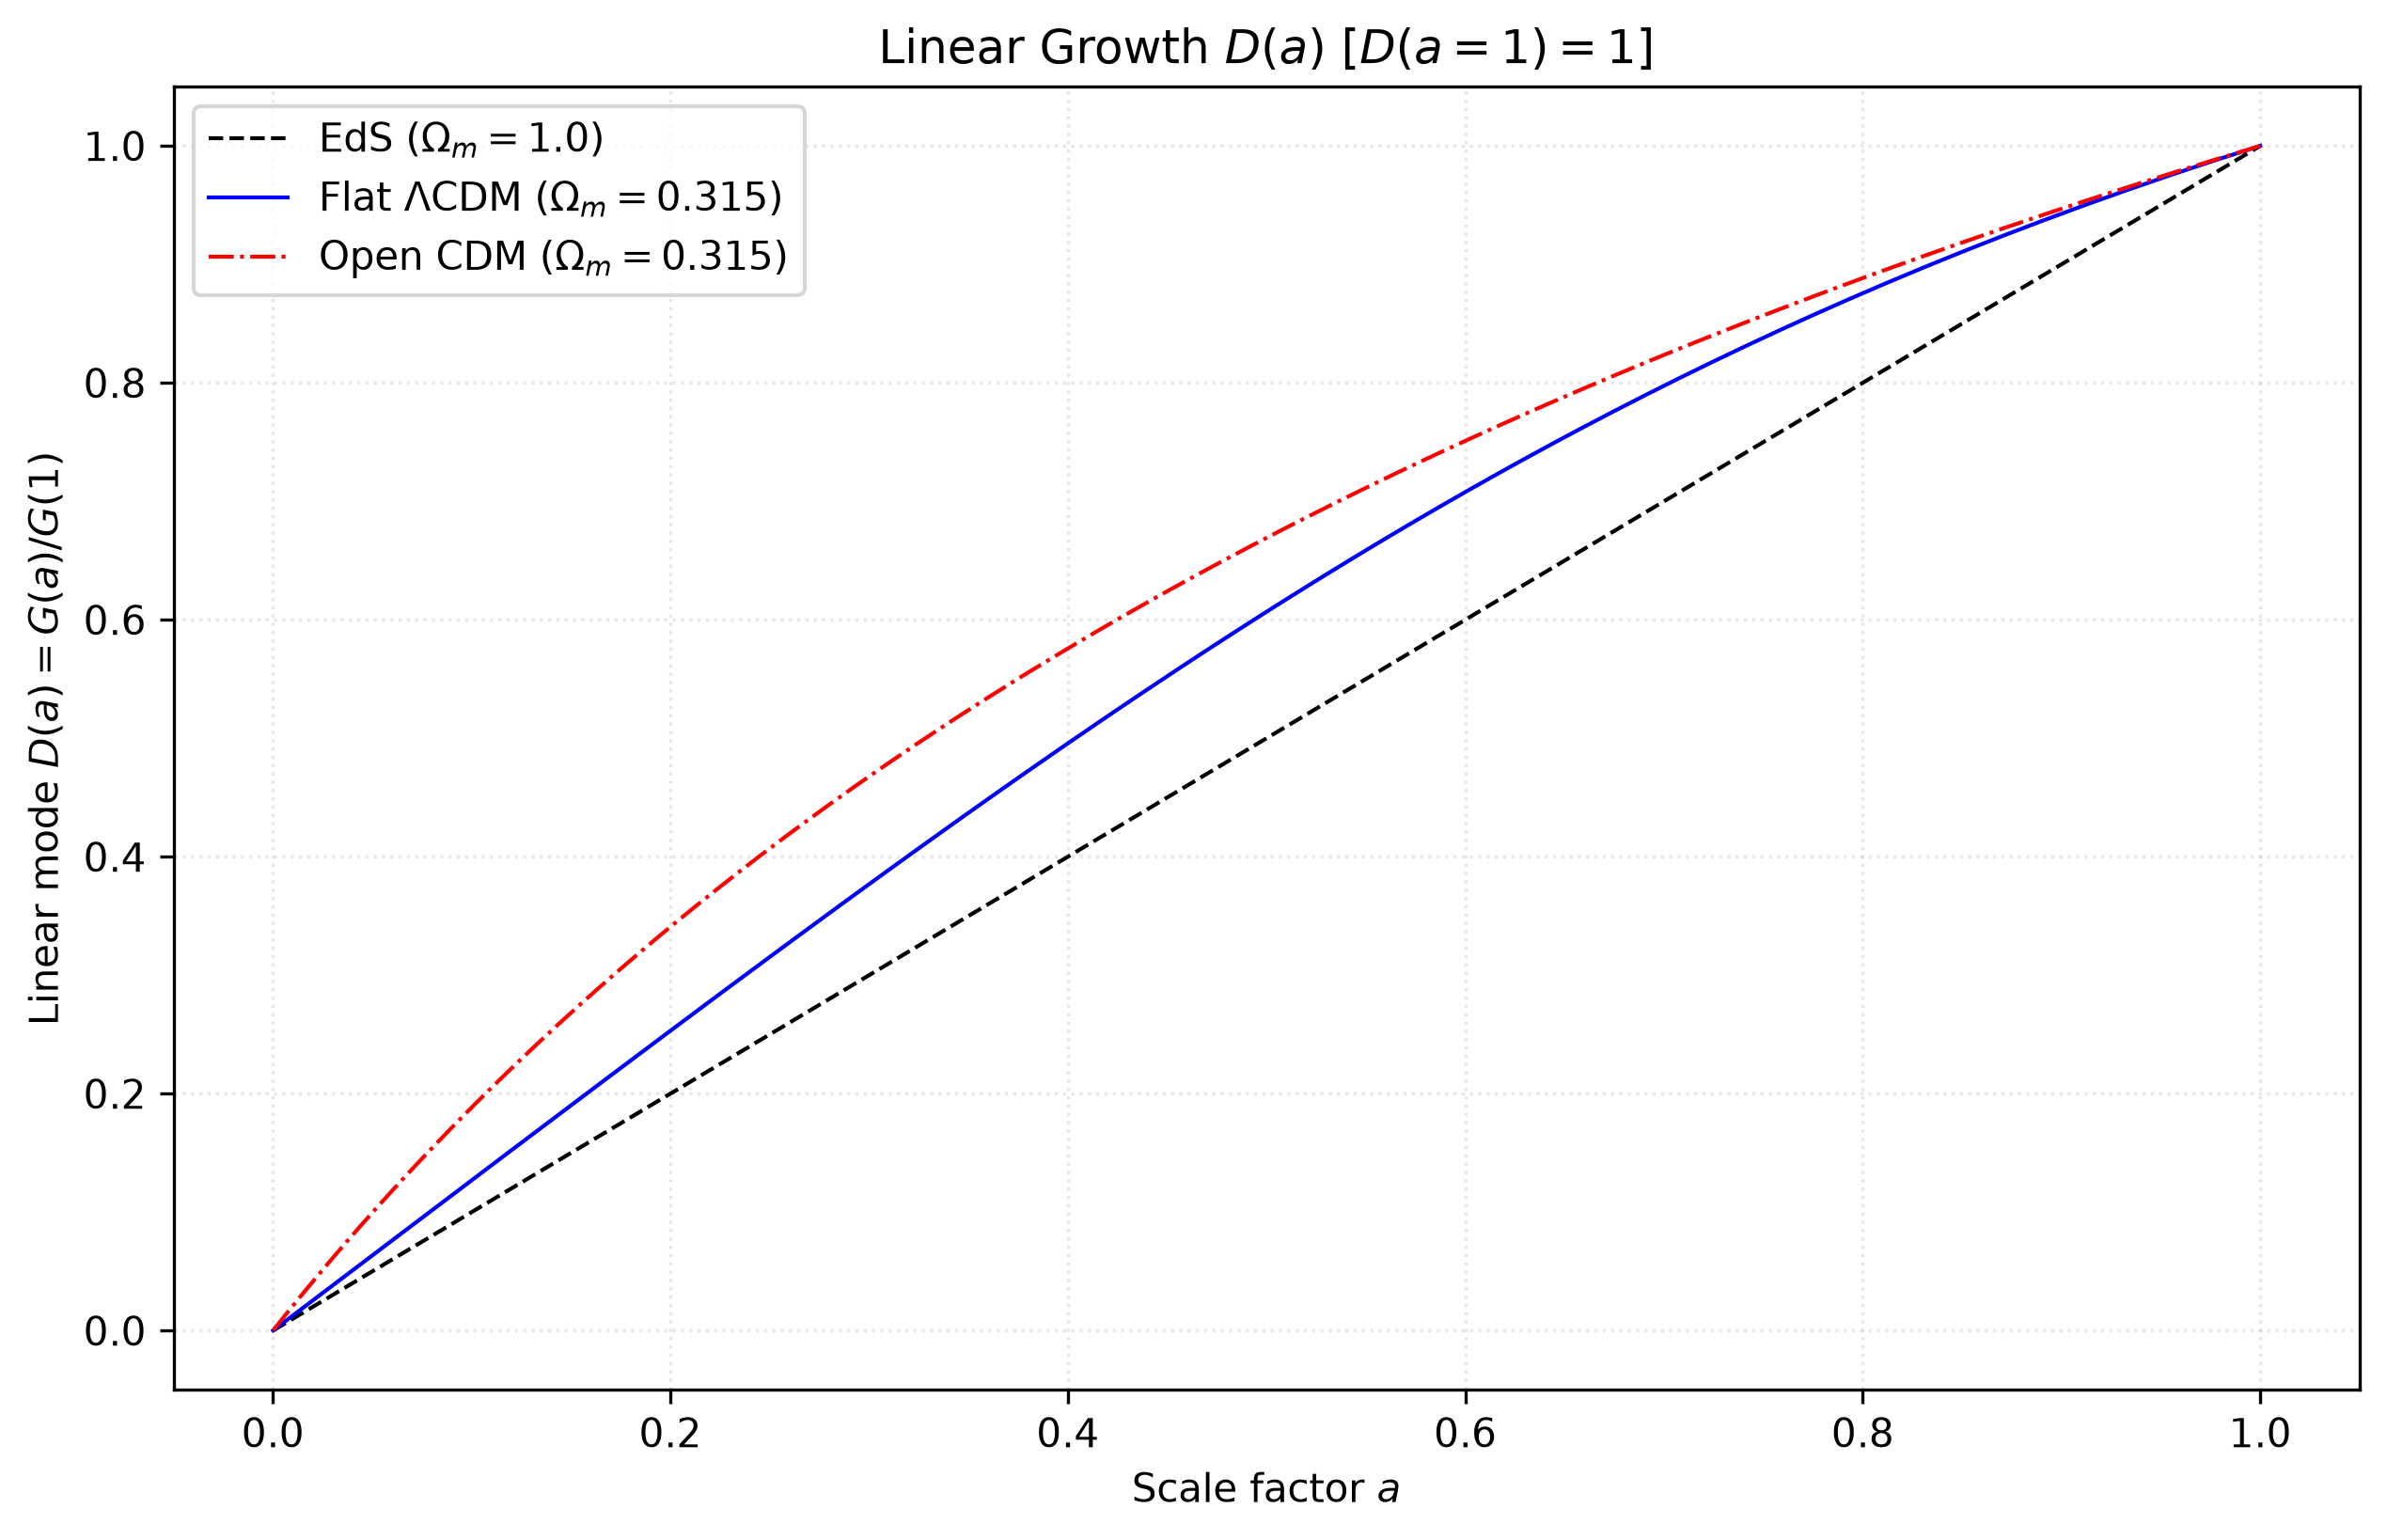
\includegraphics[width=\textwidth]{Figures/Test_20261014_164038_linear_growth.png}
        \caption{Normalized linear growth factor $D(a)$.}
        \label{fig:linear_growth_D}
    \end{subfigure}
    \hfill
    \begin{subfigure}[b]{0.48\textwidth}
        \centering
        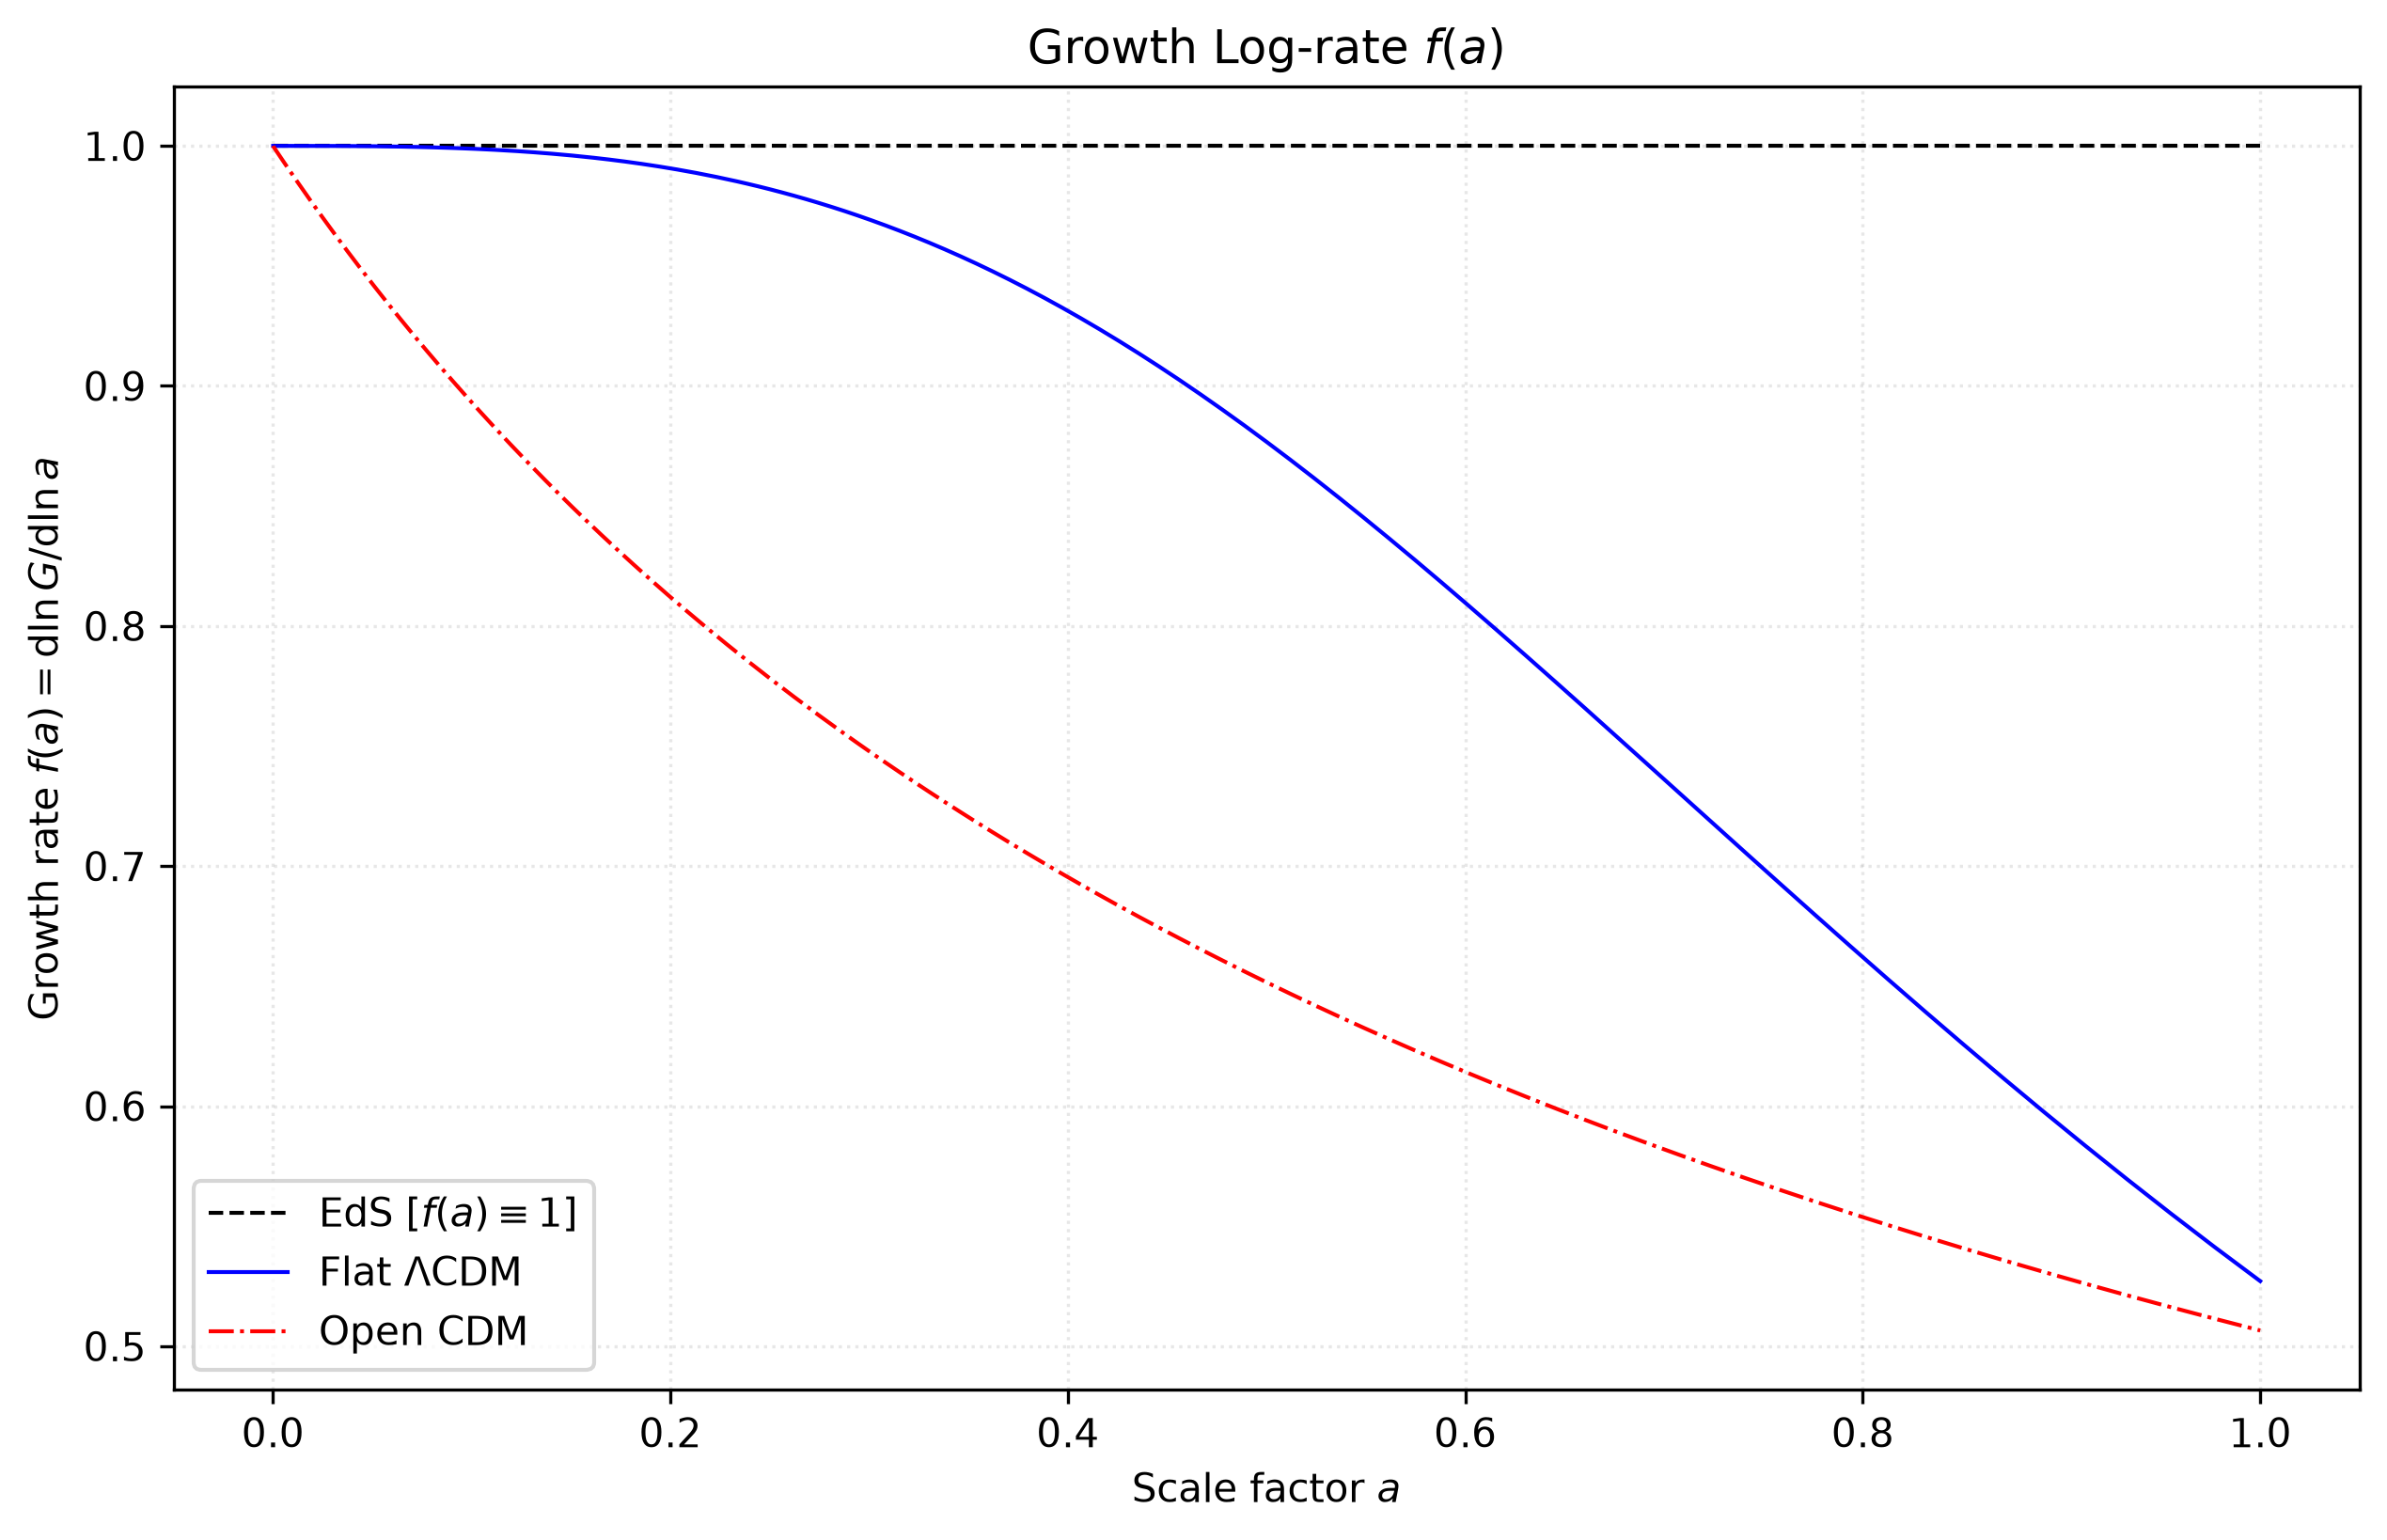
\includegraphics[width=\textwidth]{Figures/Test_20261014_164038_growth_rate.png}
        \caption{Logarithmic growth rate $f(a)$.}
        \label{fig:growth_rate_f}
    \end{subfigure}
    \caption{Evolution of linear growth observables $D(a)$ and $f(a)$ comparing EdS, flat $\Lambda$CDM, and open CDM models from $a_i = 10^{-4}$ to $a = 1.0$.}
    \label{fig:linear_growth_plots}
\end{figure}

\subsubsection{Quadrature vs. ODE Solver Benchmark}

To independently confirm the accuracy of the adaptive ODE solver (\texttt{solve\_ivp}), the unnormalized growth function $G(a)$ was evaluated via quadrature integration. 
The relative error between the ODE solution $G_{\mathrm{ODE}}(a)$ and the quadrature integration $G_{\mathrm{quad}}(a)$ across the interval $a \in [10^{-4}, 1.0]$ was measured at
    \begin{equation}
        \frac{|G_{\mathrm{ODE}}(a=1) - G_{\mathrm{quad}}(a=1)|}{G_{\mathrm{quad}}(a=1)} = 2.124 \times 10^{-7},
    \end{equation}
confirming excellent agreement between the two independent integration methods, as shown in Figure~\ref{fig:quadrature_validation}.
    \begin{figure}[htbp]
        \centering
        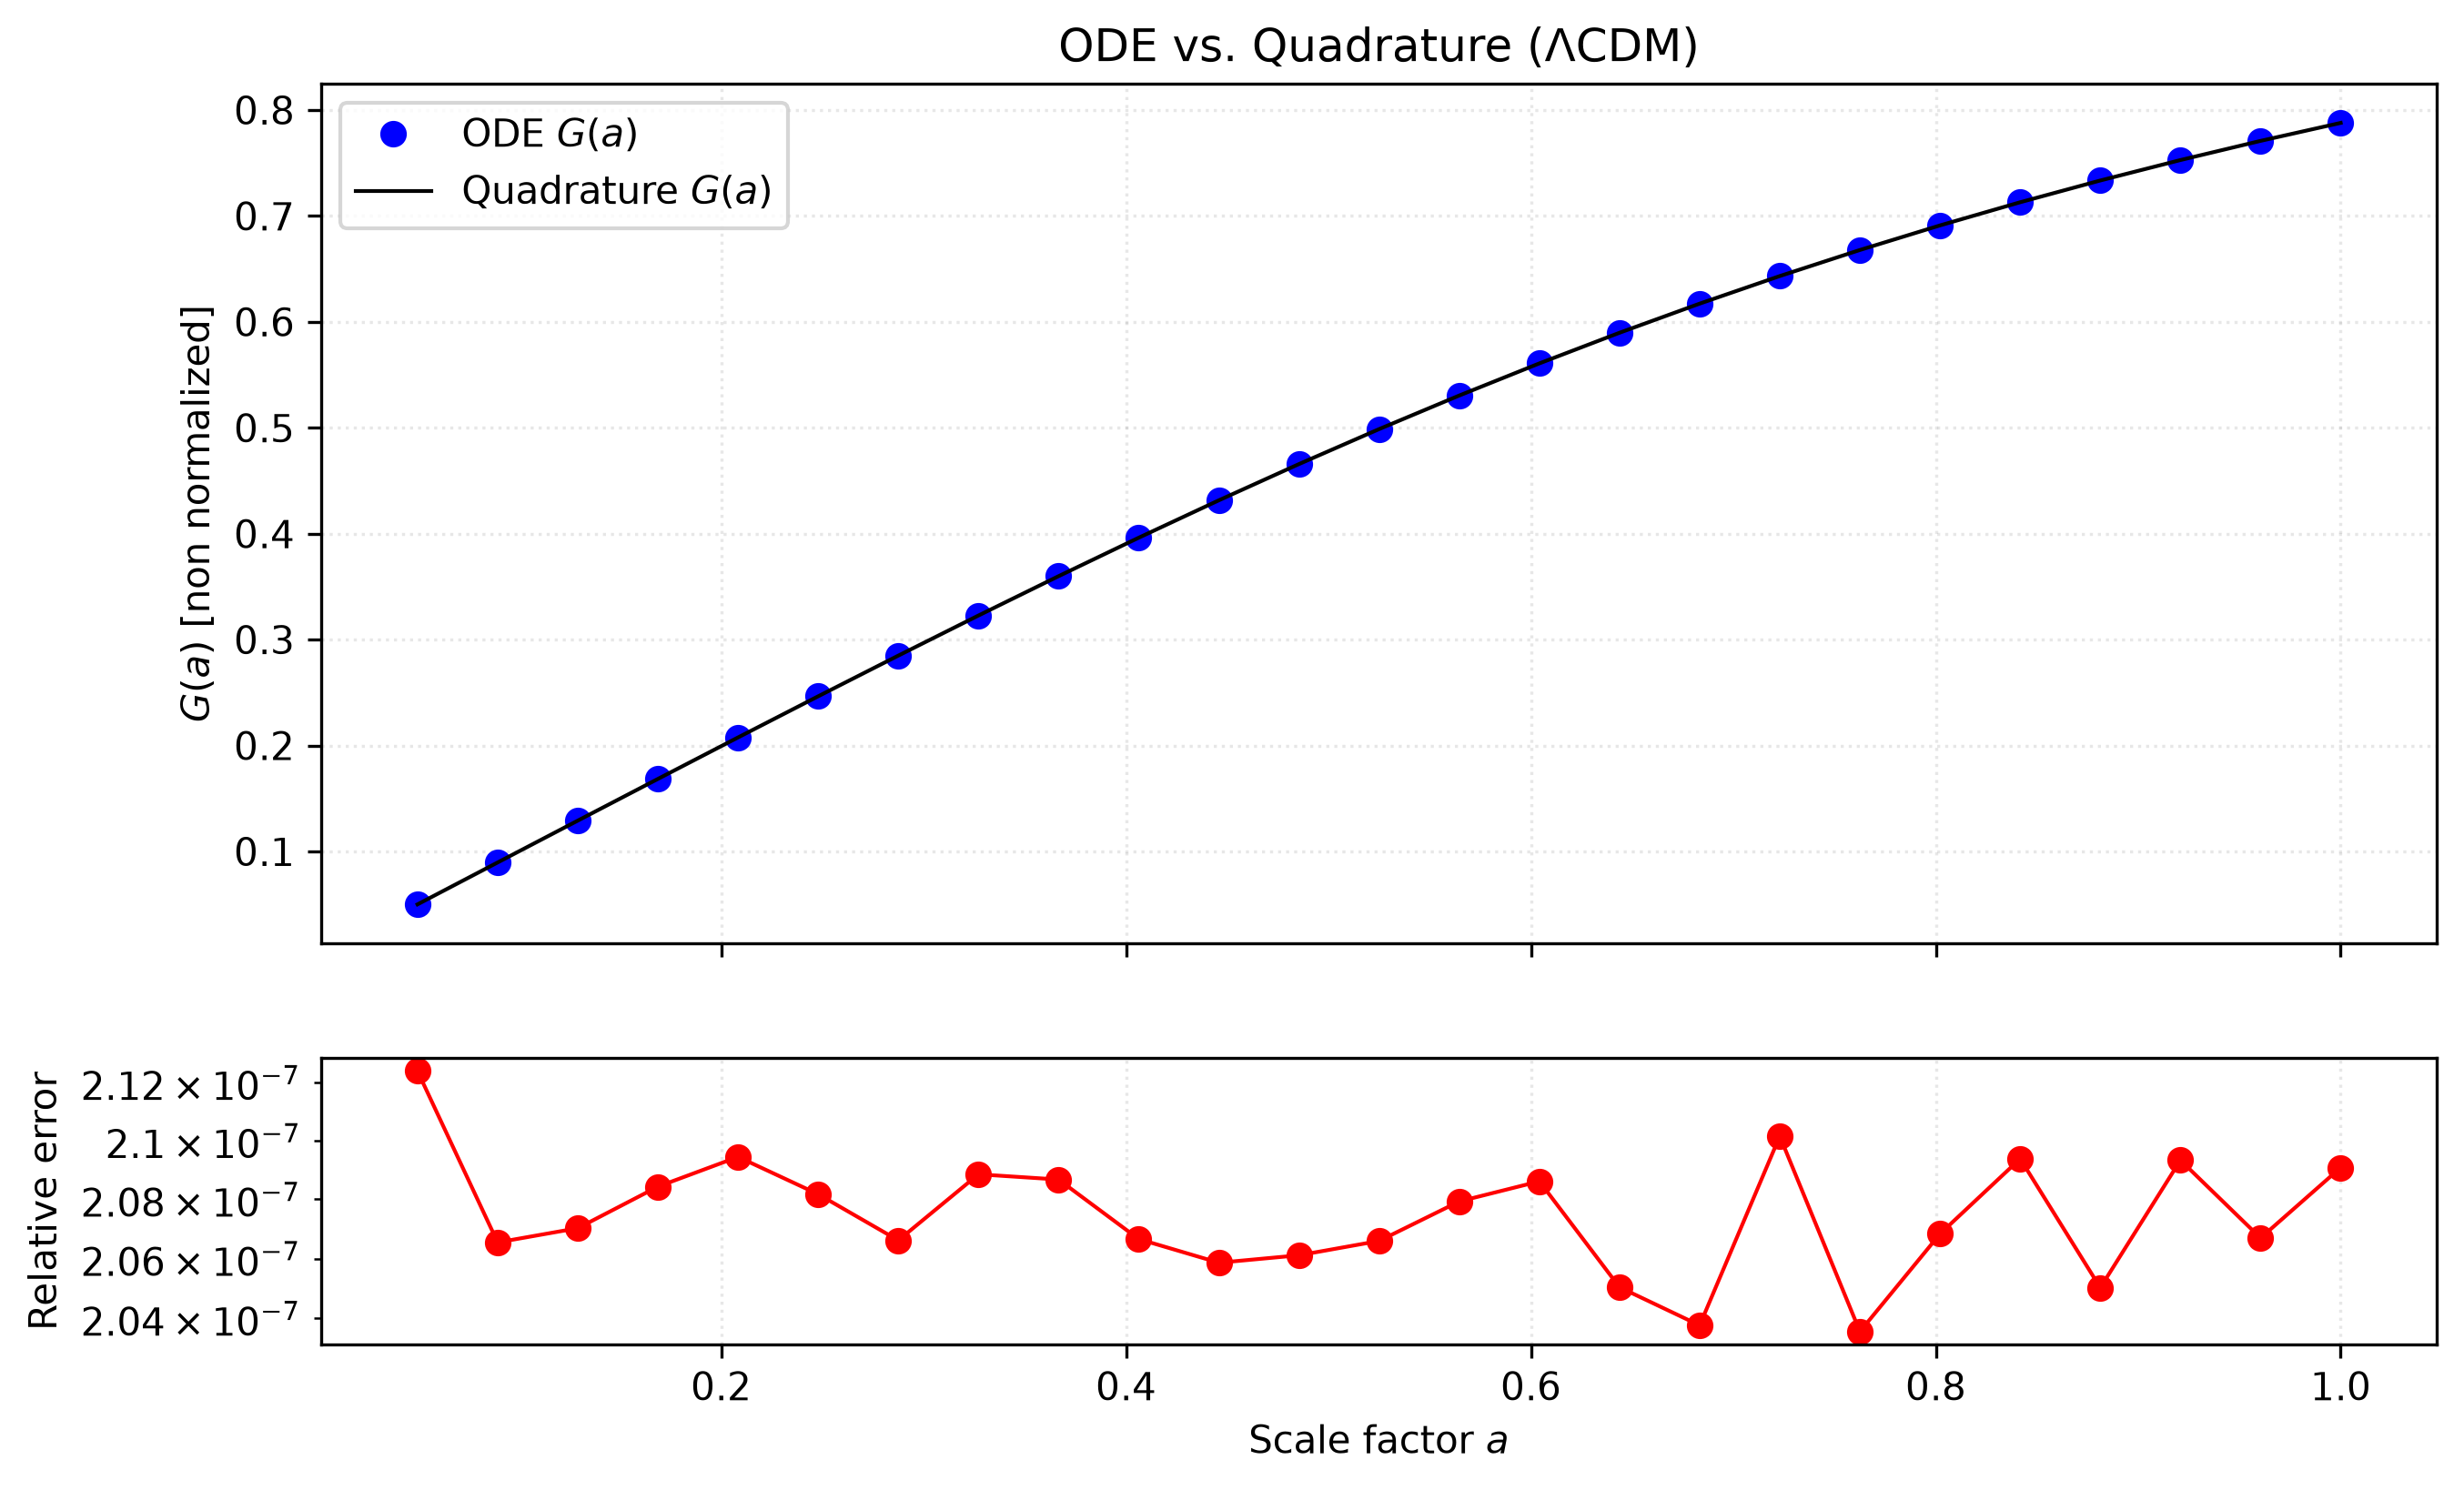
\includegraphics[width=0.9\textwidth]{Figures/Test_20261014_164038_quadrature_ODE_validation.png}
        \caption{Relative error profile comparing $G(a)$ computed via ODE integration (\texttt{solve\_ivp}) against quadrature evaluation across $a \in [10^{-4}, 1.0]$.}
        \label{fig:quadrature_validation}
    \end{figure}

\subsubsection{Initial Scale Factor and Solver Tolerance Sensitivity Analysis}

To separate initial-mode transient errors from ODE solver tolerances, we systematically varied the starting scale factor $a_i \in \{10^{-3}, 10^{-4}, 10^{-5}\}$ and adaptive integration tolerances $(\mathrm{rtol}, \mathrm{atol}) \in \{(10^{-6}, 10^{-8}), (10^{-8}, 10^{-10}), (10^{-10}, 10^{-12})\}$.

Table~\ref{tab:sensitivity_analysis} displays the stability of the observables $D(a=1)$ and $f(a=1)$ in flat $\Lambda$CDM under these varying numerical controls.
    \begin{table}[htbp]
        \centering
        \caption{Sensitivity analysis of growth observables $f(a=1)$ and $D(a=1)$ in flat $\Lambda$CDM as a function of initial scale factor $a_i$ and integration tolerances $(\mathrm{rtol}, \mathrm{atol})$. 
        Relative errors in $f(1)$ are computed against the highest precision baseline.}
        \label{tab:sensitivity_analysis}
        \begin{tabular}{ccccc}
            \hline\hline
            $a_i$ & \textbf{Tolerances} $(\mathrm{rtol}, \mathrm{atol})$ & $f(a=1)$ & $D(a=1)$ & \textbf{Rel. Error in } $f(1)$ \\
            \hline
            $1.0 \times 10^{-3}$ & $(10^{-6}, 10^{-8})$  & $0.52710275$ & $1.00000000$ & $0.00 \times 10^0$ \\
            $1.0 \times 10^{-3}$ & $(10^{-8}, 10^{-10})$ & $0.52710320$ & $1.00000000$ & $8.54 \times 10^{-7}$ \\
            $1.0 \times 10^{-3}$ & $(10^{-10}, 10^{-12})$& $0.52710320$ & $1.00000000$ & $8.62 \times 10^{-7}$ \\
            \hline
            $1.0 \times 10^{-4}$ & $(10^{-6}, 10^{-8})$  & $0.52710281$ & $1.00000000$ & $1.24 \times 10^{-7}$ \\
            $1.0 \times 10^{-4}$ & $(10^{-8}, 10^{-10})$ & $0.52710320$ & $1.00000000$ & $8.54 \times 10^{-7}$ \\
            $1.0 \times 10^{-4}$ & $(10^{-10}, 10^{-12})$& $0.52710320$ & $1.00000000$ & $8.62 \times 10^{-7}$ \\
            \hline
            $1.0 \times 10^{-5}$ & $(10^{-6}, 10^{-8})$  & $0.52710276$ & $1.00000000$ & $2.71 \times 10^{-8}$ \\
            $1.0 \times 10^{-5}$ & $(10^{-8}, 10^{-10})$ & $0.52710320$ & $1.00000000$ & $8.54 \times 10^{-7}$ \\
            $1.0 \times 10^{-5}$ & $(10^{-10}, 10^{-12})$& $0.52710320$ & $1.00000000$ & $8.62 \times 10^{-7}$ \\
            \hline\hline
        \end{tabular}
    \end{table}
    
The sensitivity study demonstrates that the normalized growth factor $D(a=1) = 1.00000000$ remains invariant across all test conditions; the logarithmic growth rate converges to $f(a=1) = 0.52710320$ once tolerances reach $\mathrm{rtol} \le 10^{-8}$, with relative variations bounded below $10^{-6}$ across three orders of magnitude in $a_i$; and starting at $a_i \le 10^{-4}$ with tolerances $(\mathrm{rtol}, \mathrm{atol}) = (10^{-8}, 10^{-10})$ eliminates initial-mode transient contamination, providing a stable baseline for subsequent 1LPT and spherical collapse computations.